% !TeX spellcheck = cs_CZ
\begin{example}\label{fyz:fey_exam001}
  \href{http://librarian/stable.php?id=380}{Soustředné válce}: Velmi tenký nevodivý plášť 
  válce o poloměru \(b\) a délce \(L\) obklopuje dlouhý, plný nevodivý válec o poloměru \(a\) 
  a délce \(L\), kde \(b < a\). V celém objemu vnitřního válce je spojitě vyplněn
  nábojem o celkové velikosti \(+Q\). Na povrchu vnějším plášti válce je spojitě rozprostřen 
  náboj stejné velikosti, opačného znaménka \(−Q\). Oblast \(a < r < b\) je prázdná. S 
  využitím Gaussova zákona určete intenzitu elektrického pole v celém prostoru.
        
  {\centering
   \captionsetup{type=figure}
   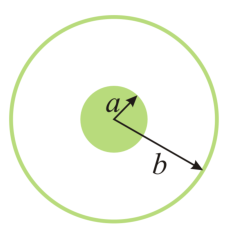
\includegraphics[width=0.3\linewidth]{fyz_fig212.pdf}
   \captionof{figure}{K příkladu \ref{fyz:fey_exam001}
   \label{fyz:fig212}}
  \par}
  
  \begin{enumerate}
    \item \emph{Jaká je symetrie úlohy?} Cylindrická
    \item \emph{Jaký je směr intenzity elektrického pole?} Vektor intenzity elektrické pole 
          míří v radiálním směru cylindrické vztažné soustavy, jeho velikost je konstantní na 
          cylindrických plochách s konstantním poloměrem. 
    \item \emph{Kolik různých oblastí v prostoru budeme vyšetřovat?} Budeme vyšetřovat tři 
          oblasti, uvnitř \(a\), mezi \(a\) a \(b\), vně \(b\).
    \item \emph{Pro každou oblast v prostoru zvolte Gaussovu plochu, jakou proměnnou zvolíte
          pro parametrizaci těchto ploch? Jaké jsou obory hodnot této proměnné?}
          V každé oblasti budeme používat válcové plochy o poloměru \(r\) a výšce \(h\), 
          které jsou souosé se skutečnými válci. Plochu budeme popisovat poloměrem \(r\), 
          jehož obor hodnot je interval \(\left\langle 0,\infty\right)\).
    \item \emph{Pro oblast \(r < a\) spočítejte tok Gaussovou plochou, kterou jste si 
          vybrali. Ve vyjádření by jste měli mít i neznámou intenzitu elektrického pole.} Obě 
          podstavy Gaussova válce nebudou přispívat k celkovému toku plochou (ze         
          symetrie je pole rovnoběžné s touto plochou). Tok pláštěm válce tak je
          \begin{equation*}
            \Phi_E = \oiint\vec{E}\dd{S} = 2\pi r h E.
          \end{equation*}
    \item \emph{Pro oblast r < a spočítejte náboj uzavřený ve zvolené Gaussově ploše.}
          Ve vnitřním válci je náboj homogenně rozložen. Náboj uzavřený v Gaussově ploše   
          můžeme vyjádřit dvěma způsoby: (1) jako objemový podíl uzavřený v ploše nebo (2)   
          využitím objemové nábojové hustoty \(\varrho\). Výpočet je proveden oběma způsoby:
          \begin{enumerate}
            \item \(Q_{in} = \dfrac{V_{in}}{V_{total}}Q = \dfrac{r^2h}{a^2L}Q\)
            \item \(\varrho = \dfrac{Q}{L\pi a^2} 
                             \Rightarrow Q_{in} = \varrho\pi r^2h = \dfrac{r^2h}{a^2L}Q
                  \)
          \end{enumerate}
    \item \emph{Pro oblast \(r < a\) dejte podle Gaussova zákona do rovnosti vztahy z 5. a 6. 
          bodu, vyjádřete velikost intenzity elektrického pole.}
          \begin{equation*}
            2\pi r h E = \frac{1}{\varepsilon_0}\dfrac{r^2h}{a^2L}Q 
                       \Rightarrow E = \frac{Qr}{2\pi\varepsilon_0a^2L}
          \end{equation*}
          \emph{Zopakujte stejnou proceduru pro oblast \(a < r < b\), vyjádřete intenzitu
           elektrického pole jako funkci \(r\).} Náboj, který je uzavřen v ploše je 
           konstantní, se vzrůstajícím poloměrem r se však mění celková plocha válce.
          \begin{equation*}
            2\pi\,r\,h\,E = \frac{1}{\varepsilon_0}\dfrac{h}{L}Q 
                            \Rightarrow E = \frac{Q}{2\pi\varepsilon_0rL}
          \end{equation*}
    \item Zakreslete \emph{intenzitu elektrického pole} jako graf funkce v závislosti na 
          parametru, který popisoval Gaussovou plochu. Graf nakreslete pro celý prostor. 
          
           {\centering
            \captionsetup{type=figure}
            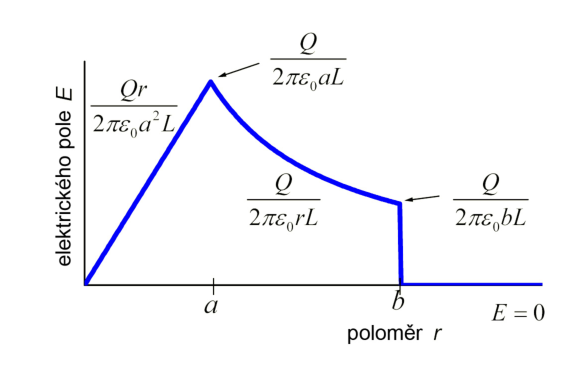
\includegraphics[width=0.9\linewidth]{fyz_fig213.pdf}
            \captionof{figure}{K příkladu \ref{fyz:fey_exam001}
            \label{fyz:fig213}}
            \par}
    \item Jaký je \emph{rozdíl potenciálů} mezi body \(r = a\) a \(r = 0\)? Tedy, kolik je
          \(\Delta V = V(a) − V(0)\)? 
          \begin{align*}
            \Delta V  = V(a) − V(0) &= -\int_0^a\vec{E}(r)\dd\vec{r}   
                                     = -\int_{0}^{a}E(r)\vec{r}\cdot\vec{r}\dd{r}    \\
                                    &= -\int_{0}^{a}\frac{Qr}{2\pi\varepsilon_0a^2L} 
                                     = -\frac{Q}{2\pi\varepsilon_0L}
          \end{align*}
    \item Jaký je rozdíl potenciálů mezi body \(r = b\) a \(r = a\)?
          \begin{align*}
            \Delta V  = V(b) − V(a) &= -\int_a^b\vec{E}(r)\dd\vec{r}   
                                     = -\int_a^b E(r)\vec{r}\cdot\vec{r}\dd{r}    \\
                                    &= -\int_a^b \frac{Q}{2\pi\varepsilon_0rL} 
                                     = -\frac{Q}{2\pi\varepsilon_0L}\ln\frac{b}{a}
          \end{align*}
          Opět je rozdíl potenciálů záporný, neboť potenciál v místě \(r = a\) je vyšší než v 
          místě \(r = b\).
  \end{enumerate}
\end{example}